% Appendix A

\chapter{Appendix A Gantt Details} % Main appendix title

\label{AppendixA} % For referencing this appendix elsewhere, use \ref{AppendixA}

Figure \ref{fig:gantt_complete} presents a detailed Gantt chart that outlines all project sub-tasks and their respective timelines, showcasing the relationships and dependencies between tasks. While parallelism could potentially provide more time for individual tasks, achieving it in this project is challenging, as noted in the main document. However, a Start-to-Start relationship is established between the task of studying a language and the implementation or environment design. This decision reflects the importance of dedicating time to the study phase while allowing for parallel progress to optimize the schedule.

For clarity, the variance column has been omitted from the chart, as its details are thoroughly addressed in the main document. Similarly, the baseline, set at the project’s inception, has been excluded to avoid unnecessary visual complexity in the diagram.

\begin{figure}
    \centering
    \frame{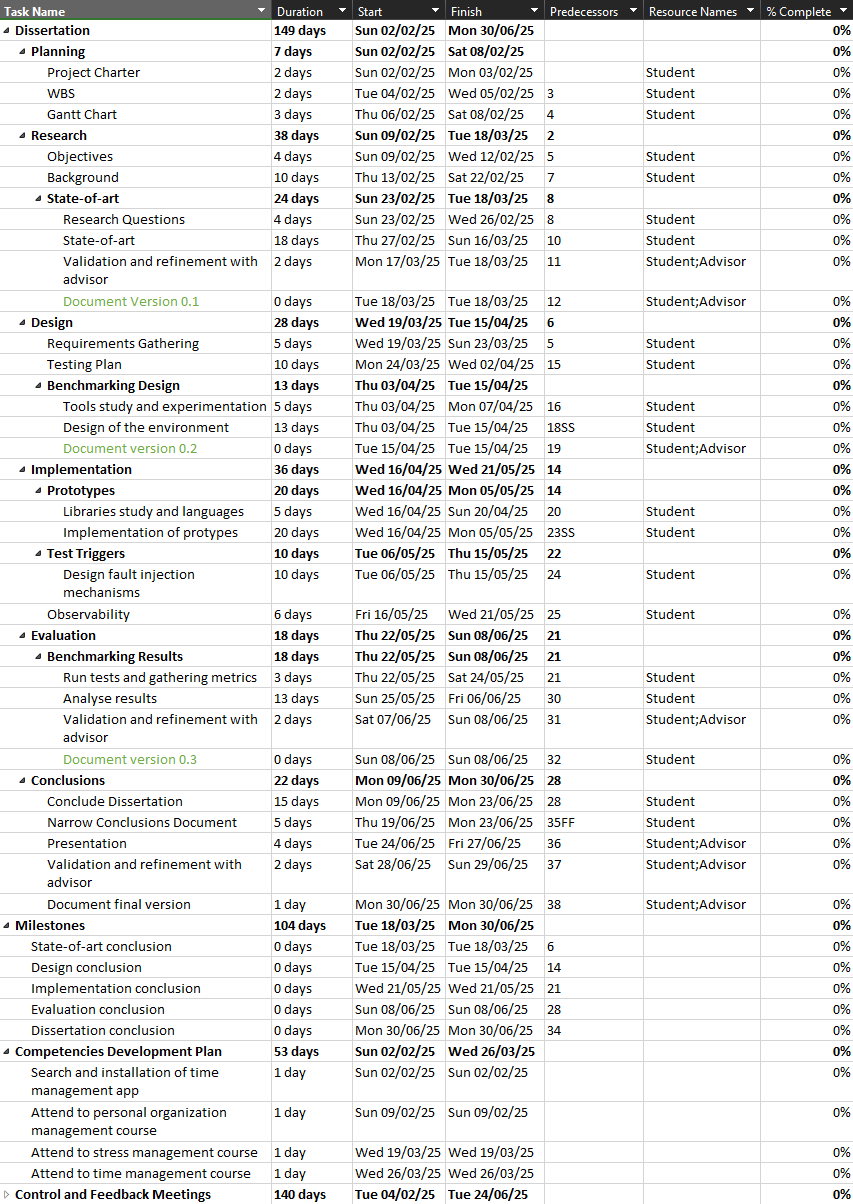
\includegraphics[width=\linewidth]{appendices/assets/gantt_complete.png}}
    \caption{Complete demonstration of the Gantt}
    \label{fig:gantt_complete}
\end{figure}